\documentclass[a4paper, 12pt]{article}

\usepackage{cmap} % поиск в PDF lusepackage[2A]{fontenc} % кодировка

\usepackage[utf8]{inputenc} % кодировка исходного текста
\usepackage[english,russian]{babel} % локализация и переносы
\usepackage{amsmath, amsfonts, amssymb, amsthm, mathtools, float}
\usepackage{ stmaryrd }

% Рисунки
\usepackage{graphicx}
\usepackage{wrapfig}

\usepackage[left=2cm,right=2cm, top=2cm,bottom=2cm,bindingoffset=0cm]{geometry}

\usepackage{longtable}

\graphicspath{pictures}

\author{Балдин Виктор}
\title{Работа 1.2.4 \\ Определении главных моментов инерции твердых тел с помощью крутильных колебаний}

\begin{document}

	\maketitle
	\section{Аннотация}
	\textbf{Цель работы:} измерить периоды крутильных колебаний рамки при различных положениях закрепленного
	в ней тела, проверить теоретическую зависимость между периодами крутильных колебаний тела
	относительно различных осей, определить моменты инерции относительно нескольких осей для каждого тела,
	по ним найти главные моменты инерции тела и посторить эллипсоид инерции.
	\bigskip\\
	\textbf{Оборудование:} установка для получения крутильных колебаний, набор исследуемых твердых тел, секундомер.

	\section{Теоретические сведения}
	Инерционные свойства твердого тела при вращении определяется
	 пространственным распределением. Оно характеризуется тензором инерции тела. Тензор инерции твердого тела
	 является симметричным тензором 2-ого ранга $J\in  T_{2}^{0}(V)$ и имеет 6 независимых компонент,
	 которые в прямоугольной декартовой системе координат выражаются как:
	\begin{equation}
	    I_{ij}=\int (\delta _{ij}r^{2}-r_{i}r_{j}) \ dm =I_{ji},
	\end{equation}
	 где $r$ — расстояния от точек до центра, относительно которого вычисляется тензор инерции,
	а $r_{i}$ — координатные компоненты соответствующих отрезков, $i$ и $j$ — номера координат (от 1 до 3).\\
	Если для какой либо системы координат все 6 компонент известны, то момент инерции тела относительно
	 произвольной оси $l$, проходящей через начало координат может быть вычислен по формуле:
	\begin{equation}
	    I_{l}=n^{j}n^{i}I_{ij}=\vec{n}^{T} I \vec{n}
	\end{equation}
	где $\vec{n}$ - единичный вектор-столбец который задает направление оси, $I$ - тензор инерции.\\
	А момент импульса $\vec  {L}$ и вращательная энергия тела $E_{\text{вращ}}$ тогда будут выражаться как:
	\begin{equation}
	    E_{\text{вращ}}={1 \over 2}\ {\vec {\omega }}^{\,T} I {\vec {\omega }} ={1 \over 2}\sum _{{ij}}\omega^{i}J_{{ij}}\omega^{j}
	\end{equation}
	\begin{equation}
	    {\vec  {L}}=I {\vec  {\omega }}, \ \ \ \ L_{i}=\sum _{j}I_{{ij}}\omega^{j}
	\end{equation}
	Отложим вдоль оси $l$ из начала координат радиус-вектор $r$
	равный по длине $1/\sqrt{I_{l}}$. Проведем множество таких отрезков, соответствующих различным направлениям оси $l$.
	 Геометрическое место концов указанных отрезков, является поверхность второго порядка - эллипсоид. Этот эллипсоид принято называть
	 эллипсоидом инерции. Он жестко связан с телом для которого он построен. Знание эллипсоида инерции позволяет найти момент инерции тела
	относительно любой оси, проходящей через центр эллипсоида. Длина отрезка $r$ будет определять момент инерции тела относительно оси $l$:
	\begin{equation}
	    I_{l} = \frac{1}{r^2}
	\end{equation}
	\begin{figure}[H]
		\centering
		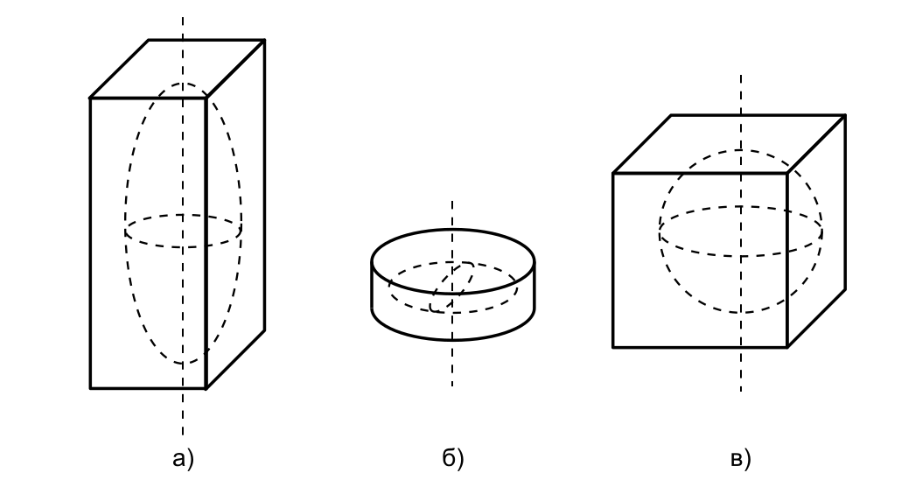
\includegraphics[scale = 0.5]{pictures/ellipsoid.png}
		\caption{Эллипсоиды вращения для разных тел}
	\end{figure}

	Как и всякий симметричный тензор второго ранга может быть диагонализован некоторой заменой координат.
	Пусть система координат, в которой он диагонализован имеет оси $Ox,Oy,Oz$, тогда эти оси совпадают с главными осями тела.
	Полученные диагональные элементы $I_{x}, I_{y}, I_{z}$ называются главными моментами инерции тела, а уравнение эллипсоида
	 инерции в этих координатах примет вид:
	\begin{equation}
	    I_{x}r^{2}_{x}+I_{y}r^{2}_{y}+I_{z}r^{2}_{z} = 1
	\end{equation}
	Крутильные колебания рамки с телом описываются уравнением:
	\begin{equation}
	    (I + I_p)\ddot{\varphi} + f \varphi = 0
	\end{equation}
	Здесь $I$ и $I_{p}$ - моменты инерции тела и рамки относительно
	 оси вращения, $\varphi$ - угол поворота рамки, меняющийся со
	временем $t$, $f$ - модуль кручения проволоки. Отсюда период этих колебаний:
	\begin{equation}
	    T = 2\pi\sqrt{\frac{I+I_{p}}{f}}
	\end{equation}
	На рисунке показано, как проходят оси вращения в параллелепипеде.
	 Оси $AA'$, $BB'$ и $CC'$ являются главными. Моменты инерции относительно
	этих осей обозначим соответственно $I_{x}, I_{y}, I_{z}$.\\

	\begin{figure}[H]
	    \begin{center}
	        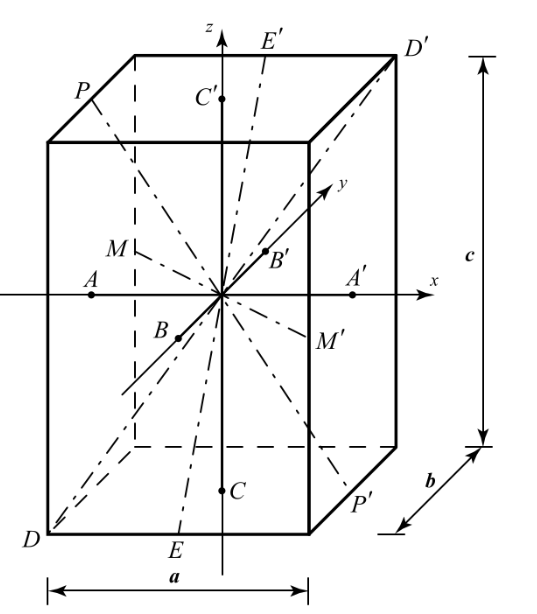
\includegraphics[scale=0.5]{pictures/kyb.png}
	        \caption{Оси вращения прямоугольного параллелепипеда}
	        \label{graphic1}
	    \end{center}
	\end{figure}

	Момент инерции $I_{D}$ при вращении относительно диагонали $DD'$ выражается
	 через главные моменты с помощью формулы:
	\begin{equation}
	    I_{d}=I_{x}\frac{a^2}{d^2}+I_{y}\frac{b^2}{d^2}+I_{z}\frac{c^2}{d^2}
	\end{equation}
	Используя связь момента инерции с периодом крутильных колебаний
	получаем соотношение между периодами колебаний относительно осей $DD'$, $EE'$,
	$MM'$ и $PP'$ с периодами крутильных колебаний относительно главных осей.
	\begin{equation}
		\begin{cases}
		(b^2+c^2)T^2_{E}=b^2 T^2_{y}+c^2 T^2_{z} \\
		(a^2+c^2)T^2_{P}=a^2 T^2_{x}+c^2 T^2_{z} \\
		(a^2+b^2)T^2_{M}=a^2 T^2_{x}+b^2 T^2_{y}
		\end{cases}
	\end{equation}

	Эти соотношения также необходимо проверить экспериментально.

 	\section{Методика измерений}
	В данной работе используется установка для измерения крутильных колебаний, приведенная
	на рисунке 3. Рамка 1 жестко соединена с проволокой 2, закрепленной вертикально в специальных
	зажимах 3, позволяющих сообщить начальное закручивание для возбуждения крутильных колебаний
	вокруг вертикальной оси.
	\begin{figure}[H]
		\centering
		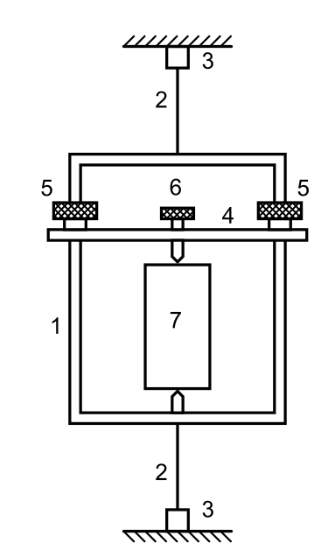
\includegraphics[scale = 0.5]{pictures/stand.png}
		\caption{Схема установки}
	\end{figure}

%
%
	\section{Используемое оборудование}
	Установка для получения крутильных колебаний, набор исследуемых твердых тел, секундомер.

%
%	\section{Результаты измерений и обработка данных}
%
%	\section{Обсуждение результатов}
%	\section{Вывод}
\end{document}
